\documentclass[../thesis/thesis.tex]{subfiles}
\begin{document}

\chapter{Literature Review}
\label{chap:litreview}

%Introduction

In this chapter, we first review the startup investment literature to develop criteria to evaluate our \gls{vc} investment screening system. We then turn our focus to determining the best techniques to use to create this system, which we break down into three intercorrelated areas: feature selection, data sources and classification algorithms.

\begin{enumerate}

\item Criteria Selection. \Gls{vc} firms review many potential investment candidates to shortlist for investment. Traditional screening methods involve referral, networking and Internet search. These screening methods are highly time-consuming and subject to human selection biases. Based on our review, we believe that a superior system can be produced and should be assessed on the basis of its efficiency, robustness, and predictive power.

\item Feature Selection. \Gls{vc} is a key driver of startup development but our understanding of factors that influence \gls{vc} firms' investment decisions and the subsequent performance of those investments is incomplete. Based on our review of the literature, we propose a hierarchical framework that includes a variety of features that have been previously indicated to be relevant to this investment screening problem. At a high-level, our framework incorporates determinants of startup potential and signals that influence investment confidence.

\item Data Sources. Startup performance is a multi-faceted problem and different data sources provide insights into different actors, relationships and attributes. Our review focuses on novel online data sources which have the potential to transform entrepreneurship and \gls{vc} research. Preliminary evidence suggests that the online startup databases CrunchBase and AngelList are promising and likely to provide a comprehensive feature set that can form the basis of our system. Other sources like PatentsView, Twitter, LinkedIn, and PrivCo are considered.

\item Classification Algorithms. Predicting startup performance is a difficult problem for humans. After all, a high percentage of even \gls{vc}-backed startups still fail. However, machine learning techniques have been recently used in other areas of finance (e.g. in the public markets) with some success. We cross-reference the characteristics of our intended dataset with the characteristics of common supervised classification algorithms. Our analyses suggest that we should expect Random Forests, Support Vector Machines and Artificial Neural Networks to be most suitable for our system.

\end{enumerate}

\section{Criteria Selection}

\Gls{vc} financing has lagged behind other forms of high finance (e.g. bond trading, loan applications, insurance) in adopting computational analytics to aid decision-making. Banks are now able to evaluate personal loan requests in minutes while \gls{vc} firms take far longer to put together deals, sometimes months. While these are markedly different forms of finance (\gls{vc} has a longer return period, larger investments, higher risk profiles), a more data-informed and analytical approach to venture finance is still foreseeable.

In this section, we provide an introduction into \gls{vc} firm strategy and review the existing state of the \gls{vc} investment process. We find that analytical tools are nascent and use of analytics in industry is limited. To date only a small handful of \gls{vc} firms have publicly declared their use of computational analytical methods in their decision making and investment selection process. We explore why the use of data mining in the \gls{vc} industry is limited and we develop criteria by which we can judge a \gls{vc} investment screening system to be successful.

\subsection{Venture Capital Industry}

Early-stage investment is a key driving force of technological innovation and is vitally important to the wider economy, especially in high-growth and technology intensive industries (e.g software, medical and agricultural technologies). \Gls{vc} is a form of private equity, a medium to long-term form of finance provided in return for an equity stake in potentially high growth companies \cite{nvca2016}. Reported US \gls{vc} investments in 2015 totalled US\$60 billion \cite{nvca2016}.

%REWRITE REQUIRED -- TOO SIMILAR TO STONE (2014)
Figure~\ref{fig:litreview:criteria:fund_structure} illustrates the typical structure of a \gls{vc} Fund. A typical fund is managed by a \gls{vc} Firm (legally referred to as a General Partner) consisting of several investment partners. The fund itself (the Limited Partnership) is essentially an investment fund raised from various institutional investors such as pension funds, university endowments and family offices (legally referred to as Limited Partners). Beyond fundraising the main responsibilities of investment partners (also referred to as General Partners) are sourcing investment opportunities, making investment decisions and taking board membership to assist the management of investee private companies (also referred to as Portfolio Companies).

\begin{figure}[!htb]
    \centering
    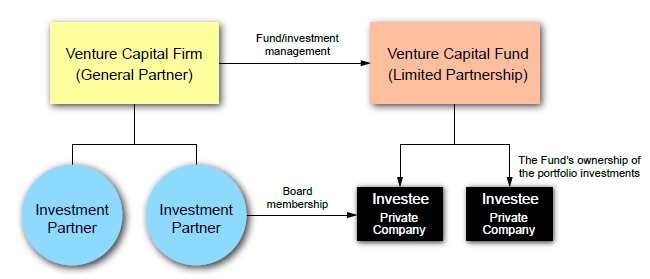
\includegraphics{../figures/litreview/fund_structure.png}
    \caption[Venture Capital fund structure]{Venture Capital fund structure.}
    \label{fig:litreview:criteria:fund_structure}
\end{figure}

\subsection{Venture Capital Firm Strategy}

Typically, \gls{vc} firms are reliant on a small number of high-risk investments to produce outsized returns through successful exit events. A common rule-of-thumb is that given a portfolio of ten startup companies: three will fail entirely, three will remain active but will not be very profitable, three will be active and profitable, and one highly successful startup will provide the investor with a multiple return on all of the investments \cite{stone2014}. In comparison to other traditional investment classes, \gls{vc} financing is heavily biased towards control at the expense of risk mitigation. Although \gls{vc} firms tend not to take majority stakes in startups, they exert their influence through significant minority stakes, board membership, their relative seniority to the company’s founders, and through leveraging their business networks \cite{fried2006}.

Despite \gls{vc} firms’, often significant, influence on the trajectory of their investments, they are still highly selective of the companies that they invest in. Although rarely reported, a small number of studies show \gls{vc} investment rates vary between 1.5-3.5\% of proposals considered \cite{stone2014}. Accordingly, traditional venture finance is a very labour intensive and time consuming process involving extensive due diligence on behalf of the investor \cite{fried1994}. The \gls{vc} investment process involves several main stages: deal origination, screening, evaluation, structuring (e.g., valuation, term sheets), and post investment activities (e.g., recruiting, financing).

\subsection{Current Venture Capital Systems}

Early-stage investment is characterised by a large number of investment candidates, high degree of uncertainty; a lack of reliable data on company performance (particularly financial performance); and a high time-cost of undertaking due diligence. This makes for a complicated origination and screening process. While referral from trusted sources (e.g., entrepreneurs, accountants, lawyers, other investors) is often used to screen opportunities, as the cost of starting businesses dramatically decreases investors are faced with an increasingly large number potential businesses and investment opportunities to assess and evaluate. Such a proliferation has led to an “information overload” problem in venture finance.

Despite evidence that \gls{vc} firms could benefit from increased use of data mining, it appears few are interested in advanced data analytics. Stone \cite{stone2014} interviewed Fred Wilson of Union Square Ventures who said: ``We have not been able to quantify [startup potential]. We haven’t even tried. Although I am sure someone could do it and they might be very successful with it. To us, the ideal founding team is one supremely talented product oriented founder and one, two, or three strong developers, and nothing else.'' Likewise, when asked, Chris Dixon of Andreessen Horowitz said: ``I’ve seen a few attempts to do it quantitatively but I think those are often flawed because the quantitatively measurable things are either obvious, irrelevant, or suffer from overfitting (finding patterns in the past that don’t carry forward in the future''.

Similarly, while recently new software tools have been developed to assist \gls{vc} firm, there is limited evidence of their adoption.

\subsection{Proposed Criteria}

Based on our review of the \gls{vc} industry and current \gls{vc} origination and screening processes, we have developed criteria on which we can evaluate our proposed system.

\begin{enumerate}

\item Efficiency. Our system must be more efficient than traditional, manual investment screening by referral and technology scan (e.g. Google search, media, databases). This means that it needs to be able to provide enough information -- both observations and features -- to be able to meet similar levels of accuracy.

\item Robustness. Our system must be robust enough to be reliable over time. The system must provide a generalised, robust solution for investors that does not require significant technical knowledge to use, and is not overfitted to a specific time-period or data source.

\item Predictive Power. Our system must be consistently accurate at identifying a variety of high-potential investment candidates. The system should be robust to different forecast windows (i.e. exit in three years from now) as \gls{vc} firms make investment decisions with different periods so they can strategically manage the investment horizons of their funds.

\end{enumerate}

\section{Feature Selection}

Our understanding of the factors that influence \gls{vc} investment decisions and the subsequent performance of those investments is incomplete. We believe a diverse range of features is critical to developing accurate models of startup performance and investment decisions.

Prior work focuses on basic company features (e.g. the headquarters' location, the age of the company) for startup investment predictive models \cite{beckwith2016, gimmon2010}. Semantic text features (e.g. patents, media) \cite{hoenen2014, yuan2016} and social network features (e.g. co-investment networks) \cite{werth2013, cheng2016, yu2015} may also predict startup investment. We expect a model that includes semantic text and social network features alongside basic company features could lead to better startup investment prediction.

We propose a conceptual framework that builds upon previous work to ensure that we include a comprehensive and relevant set of features in our investment screening system.  Ahlers et al. \cite{ahlers2015} developed a conceptual framework for funding success on equity crowdfunding platforms. Their framework has two factors: venture quality and level of uncertainty. The first factor is based on work by Baum and Silverman \cite{baum2004} that suggests key determinants of startup potential are human capital, alliance (social) capital, and intellectual (structural) capital. The second factor is based on investors' confidence in their estimation of startup potential.

We seek to generalise Ahlers' framework~\cite{ahlers2015} beyond equity crowdfunding. While the first factor of Ahlers' framework (venture quality) applies to startups of all stages, Ahlers operationalise their second factor with respect to whether startups offer an equity share in their crowdfunding, and whether they provide financial projections. These features are specific to equity crowdfunding. We propose an extension of Ahlers' framework that generalises and develops this second factor. We describe investment confidence as a product of third party validation, historical performance and contextual cues. Our proposed framework is depicted in Figure~\ref{fig:litreview:theory:framework}.

\begin{figure}[!htb]
    \centering
    
\begin{forest}
    forked edges,
    for tree={
        grow=west,
        align=center,
        l sep = 2cm,
        fork sep = 1cm,
        child anchor=east,
        anchor=base east,
        tier/.pgfmath=level(),
        edge={<-, thick},
        every node={rectangle,draw=black}
    }
[Startup\\Investment,
    [Startup\\Potential,
        [Human Capital]
        [Social Capital]
        [Structural Capital]
    ]
    [Investment\\Confidence,
        [Third Party Validation]
        [Historical Performance]
        [Contextual Cues]
    ]
]
\end{forest}

    \caption[Conceptual framework for startup investment.]{Proposed conceptual framework for startup investment. We adapt the framework proposed by Ahlers et al.~\cite{ahlers2015}, originally based on work by Baum and Silverman~\cite{baum2004}. For an extended version of this framework, please refer to Figure~\ref{fig:litreview:features:framework_details}.}
    \label{fig:litreview:features:framework_simple}
\end{figure}

Next, we must operationalise this conceptual framework into features that we can incorporate into our machine learning model. Table~\ref{fig:litreview:features:summary} shows a review of features tested in previous studies of startup investment. In Appendix~\ref{appendix:feature_summary}, we describe each of these features and outline theoretical and empirical evidence that justify their inclusion in our conceptual framework.

\begin{table}[!htb]
    \centering
    \scalebox{1}{
        
\newcommand{\factor}[1]{\hspace{-4em}#1}
\newcommand{\group}[1]{\hspace{-2em}#1}

\begin{tabular}{>{\hspace{4em}}lll}
\toprule
\multicolumn{1}{l}{Features} & \multicolumn{2}{c}{Results from Studies} \\
\cmidrule(lr){2-3}
 & Significant & Non-Significant \\
\midrule
\factor{Startup Potential} \\
      \group{Human Capital} \\
            Founder Capabilities
                  & \cite{beckwith2016,an2015,gimmon2010}
                  & \cite{shan2014,conti2013} \\
            Advisor Capabilities
                  & \cite{baum2004}
                  & \cite{ahlers2015,an2015} \\
            Executive Capabilities
                  & \cite{beckwith2016,an2015,conti2013}
                  & \cite{ahlers2015} \\
      \group{Social Capital} \\
            Strategic Alliances
                  & \cite{baum2004}
                  & - \\
            Social Influence
                  & \cite{beckwith2016,an2015,cheng2016,yu2015}
                  & - \\
      \group{Structural Capital} \\
            Patent Filings
                  & \cite{hoenen2014,hsu2008,baum2004}
                  & \cite{ahlers2015,gimmon2010} \\
\factor{Investment Confidence} \\
      \group{Third Party Validation} \\
            Investment Record
                  & \cite{ahlers2015,beckwith2016,croce2016,hoenen2014,conti2013}
                  & - \\
            Investor Reputation
                  & \cite{an2015,werth2013,hsu2008}
                  & \cite{hoenen2014} \\
            Media Coverage
                  & \cite{beckwith2016}
                  & \cite{an2015} \\
      \group{Historical Performance} \\
            Financial Performance
                  & \cite{beckwith2016,baum2004}
                  & - \\
            Non-Financial Performance
                  & \cite{an2015,gimmon2010}
                  & \cite{hoenen2014} \\
      \group{Contextual Cues} \\
            Industry Performance
                  & \cite{shan2014,croce2016,gimmon2010}
                  & \cite{beckwith2016,conti2013} \\
            Broader Economy
                  & \cite{beckwith2016,croce2016,hoenen2014,conti2013,hsu2008}
                  & \cite{shan2014,ahlers2015} \\
            Local Economy
                  & \cite{shan2014,beckwith2016,croce2016,gimmon2010,hoenen2014}
                  & - \\
\bottomrule
\end{tabular}

    }
    \caption[Features relevant to startup investment]{Features relevant to startup investment. We review thirteen empirical studies that investigate drivers of startup investment. For each study, we note whether included features have a significant effect on the startup investment model. We classify identified features according to our proposed conceptual framework.}
    \label{fig:litreview:features:summary}
\end{table}

Feature selection is critical to the success of our proposed conceptual framework. In this section, we have built on the framework proposed by Ahlers et al. \cite{ahlers2015} in several ways. First, our framework generalises the ``Investment Confidence'' factor for startups seeking any type of investment (not just equity crowdfunding). Second, our framework has greater depth. Where Ahlers uses one or two features for each factor in their model (e.g. ``\% Nonexecutive board'' represents ``Social (alliance) capital''), we perform a review of many features employed in this area and perform a higher degree of classification. For example, in our proposed framework ``Social (alliance) capital'' is composed of ``Social influence'' and ``Strategic alliances'', each of which will also be composed of several features (e.g. ``Twitter followers'', ``Average Tweets per day'').

\section{Data Sources}

Predicting startup investment and performance is a complex and difficult task. There are many features that can influence startup investment decisions. Capturing the diversity of these features is critical to developing accurate models. Accordingly, this task will likely involve data collection from multiple data sources. Appropriate selection of these data sources is important because different data sources provide insights into different actors, relationships and attributes.

Previous studies in this field have been limited by data sources restricted in sample size. Most studies have samples of fewer than 500 startups \cite{ahlers2015, gimmon2010}, or between 500 and 2,000 startups \cite{hoenen2014, yu2015, an2015, werth2013, croce2016}, and only a few have large scale samples (more than 100,000 startups) \cite{shan2014, cheng2016}. Sample size is more critical to model development than the sophistication of machine learning algorithms or feature selection \cite{caruana2008}. Startups databases (e.g. CrunchBase) and social networks (e.g. Twitter) offer larger data sets than those previously studied. We expect data collected from these sources will lead to the discovery of additional features and higher accuracy in startup investment prediction.

In Table~\ref{fig:litreview:sources:summary}, we outline the characteristics of relevant data sources and how they could contribute to our chosen features. In this section, we describe desirable characteristics of data sources for this task, review potentially relevant data sources, and ultimately determine which data sources are most likely to suit the characteristics of this task.

\afterpage{
    \clearpage
        \begin{sidewaystable}[!htbp]
            \centering
            \scalebox{0.8}{
                
\newcommand{\type}[1]{\hspace{-6em}#1}
\newcommand{\factor}[1]{\hspace{-4em}#1}
\newcommand{\group}[1]{\hspace{-2em}#1}

\begin{tabular}{>{\hspace{6em}}lcccccc}
\toprule
\multicolumn{1}{l}{Properties} & \multicolumn{2}{c}{Startup Databases} & \multicolumn{2}{c}{Social Media} & \multicolumn{2}{c}{Other Sources}\\
\cmidrule(lr){2-3} \cmidrule(lr){4-5} \cmidrule(lr){6-7}
 & CrunchBase & AngelList & LinkedIn & Twitter & PatentsView & PrivCo \\
\midrule
\type{Features} \\
      \factor{Startup Potential} \\
            \group{Human Capital} \\
                  Founders' Capabilities %DONE
                        & \cmark & \cmark
                        & \cmark\cmark & \xmark
                        & \xmark & \xmark \\
                  NED Capabilities %DONE
                        & \cmark & \cmark
                        & \cmark\cmark & \xmark
                        & \xmark & \xmark \\
                  Staff Capabilities %DONE
                        & \cmark & \cmark
                        & \cmark\cmark & \xmark
                        & \xmark & \xmark \\
            \group{Social Capital} \\
                  Social Influence %DONE
                        & \cmark & \cmark\cmark
                        & \cmark\cmark & \cmark\cmark
                        & \xmark & \xmark \\
                  Strategic Alliances %DONE
                        & \cmark & \cmark
                        & \xmark & \xmark
                        & \cmark & \xmark \\
            \group{Structural Capital} \\
                  Patent Filings %DONE
                        & \xmark & \xmark
                        & \xmark & \xmark
                        & \cmark\cmark & \xmark \\
      \factor{Investment Confidence} \\
            \group{Third Party Validation} \\
                  Investment Record
                        & \cmark\cmark & \cmark\cmark
                        & \xmark & \xmark
                        & \xmark & \cmark \\
                  Investor Reputation
                        & \cmark & \cmark\cmark
                        & \cmark & \xmark
                        & \xmark & \xmark \\
                  Media Coverage
                        & \cmark\cmark & \cmark
                        & \xmark & \cmark
                        & \xmark & \xmark \\
                  Awards and Grants
                        & \cmark & \xmark
                        & \xmark & \xmark
                        & \xmark & \xmark \\
            \group{Historical Performance} \\
                  Financial Performance
                        & \xmark & \xmark
                        & \xmark & \xmark
                        & \xmark & \cmark\cmark \\
                  Non-Financial Performance
                        & \cmark\cmark & \cmark\cmark
                        & \cmark & \xmark
                        & \xmark & \cmark \\
            \group{Contextual Cues} \\
                  Competitor Performance
                        & \cmark & \cmark
                        & \xmark & \xmark
                        & \xmark & \xmark \\
                  Broader Economy
                        & \cmark & \cmark
                        & \xmark & \xmark
                        & \xmark & \xmark \\
                  Local Economy
                        & \cmark & \cmark
                        & \xmark & \xmark
                        & \xmark & \xmark \\
\type{Ease of Use} \\
      \factor{Cost Effective}
            & \cmark & \cmark\cmark
            & \cmark & \xmark
            & \cmark\cmark & \xmark \\
      \factor{Time Efficient}
            & \cmark\cmark & \cmark\cmark
            & \xmark & \cmark\cmark
            & \cmark\cmark & \xmark \\
      \factor{Accurate Data}
            & \cmark & \cmark
            & \cmark\cmark & \cmark\cmark
            & \cmark\cmark & \cmark\cmark \\
      \factor{Large Data Set}
            & \cmark\cmark & \cmark\cmark
            & \cmark\cmark & \cmark\cmark
            & \cmark\cmark & \cmark \\
\bottomrule
\end{tabular}

            }
            \caption[Data sources relevant to startup investment]{Data sources relevant to startup investment. We review six data sources commonly used in entrepreneurship research for their suitability for our startup investment task. We evaluate data sources for their ability to provide relevant features for our analyses and for their ease of use in data collection. We exclude offline sources from our analyses. Ratings are: \protect\xmark~=~poor, \protect\cmark~=~satisfactory, \protect\cmark\protect\cmark~=~good.}
            \label{fig:litreview:sources:summary}
        \end{sidewaystable}
    \clearpage
}

\subsection{Source Characteristics}

Entrepreneurship research is transforming with the availability of online data sources: databases, websites and social networks. Entrepreneurship studies have historically relied on surveys and interviews for data collection. Measures of human capital (e.g. founders' capabilities), strategic alliances, and financial performance are difficult to capture elsewhere. However, the trade-off for access to these features is that surveys and interviews are time-consuming and costly to implement. While online surveys address some of these issues, it is still difficult to motivate potential participants to contribute. Online data sources like startup databases and social networks are efficient because collecting data is a secondary function of users interacting with these sources. Researchers can also collect data from these sources automatically and at scale. For these reasons, we only consider online data sources for inclusion in this study, specifically crowd-sourced startup databases (e.g. CrunchBase, AngelList), social networks (e.g. Twitter, LinkedIn), government patent databases (e.g. PatentsView) and private company intelligence providers (e.g. PrivCo). In the following section we review the characteristics of each of these data sources commonly used in entrepreneurship research.

\subsubsection{Databases}

Databases play a critical role in understanding the startup ecosystem, aggregating information about startups, investors, media and trends. Most startup databases are closed systems that require commercial licenses (e.g. CB Insights, ThomsonOne, Mattermark). CrunchBase and AngelList are two crowd-sourced and free-to-use alternatives. AngelList’s primary function is as an equity crowdfunding platform but it has a data-sharing agreement with CrunchBase which results in significant overlap between the two sources. CrunchBase and AngelList provide free Application Program Interfaces (API) for academic use. Crawlers can be developed to traverse these APIs and collect data systematically. The advantages of crawlers are that they can selectively collect data from nodes with specific attributes, collect random samples, or traverse the data source indefinitely, updating entries as new data becomes available. CrunchBase also provides pre-formatted database snapshots which allows easier access to the data set. The crowd-sourced nature of CrunchBase and AngelList has advantages and limitations . The key advantages are that access to the databases is free and the dataset is relatively comprehensive. The limitations are that both CrunchBase and AngelList have relatively sparse profiles (i.e. limited depth), particularly for unpopular startups. Both CrunchBase and AngelList also have error-checking provisions (including machine reviews and social authentication) to prevent and remediate inaccurate entries but there is still a greater chance for error. Comparing CrunchBase and AngelLIst, CrunchBase tends to have more comprehensive records of funding rounds \cite{cheng2016} and media coverage but AngelList also has a social network element where users can `follow’ each other - in a similar way to Twitter.

\subsubsection{Social Networks}

Social networks provide an interesting perspective into the process of opportunity discovery and capitalisation that characterises entrepreneurship. Two social networks studied in detail in entrepreneurship research are LinkedIn and Twitter. LinkedIn is a massive professional social network often used in studies of entrepreneurship for measures of employment, education and weak social links. These measures are difficult to collect elsewhere. In addition, LinkedIn can provide a measure of the professional influence of founders and investors. Unfortunately, as of May 2015, the LinkedIn API no longer allows access to authenticated users' connection data or company data \cite{trachtenberg2015}, making it difficult to use for social network analyses. Twitter is a massive social networking and micro-blogging service which is studied in entrepreneurship research because it is used by founders, investors, and customers to quickly communicate and broadcast. Twitter is a directed network where users can follow other users without gaining their permission to do so. Twitter's public API provides access to social network topological features (e.g. who follows who) and basic profile information (e.g. user-provided descriptions). However, Twitter's API only provides Tweets published within the last 7 days and access to historical Twitter data requires a commercial license \cite{puschmann2013}.

\subsubsection{Other Sources}

While startup databases and social networks provide a variety of information on startups, there are two important areas that they do not cover: patent filings and financial performance. Startups often file patents to apply for a legal right to exclude others from using their inventions. In 2015, the US Patents Office (USPTO) launched PatentsView, a free public API to allow programmatic access to their database. PatentsView holds over 12 million patent filings from 1976 onwards \cite{schultz2016}. The database provides comprehensive information on patents, their inventors, their organisations, and locations. It may be difficult to match identities across PatentsView to other data sources because registered company names (as in PatentsView) are not always the same as trading names (as elsewhere). Finding other information on startups, like financial information, is difficult. Unlike public companies, private companies are not required to file with the United States Securities and Exchange Commission (or international equivalent). Proprietary databases provide some data on private companies but commercial licenses are prohibitively expensive and have poor coverage of early-stage companies. PrivCo is one of few commercial data sources for private company business and financial intelligence. PrivCo focuses its coverage on US private companies with at least \$50-100 million in annual revenues but also has some coverage on smaller but high-value private companies (like startups) \cite{artemchik2015}.

\subsection{Source Evaluation}

Entrepreneurship and \gls{vc} research is primed to take advantage of the availability of new online data sources. We evaluated relevant data sources for their suitability to predicting startup investment. Startup databases CrunchBase and AngelList provide the most comprehensive set of features. There are small differences between the features recorded by each. CrunchBase has slightly more coverage and tracks media better but lacks AngelList's social network. At least one startup database should be used and either are satisfactory. Of the other data sources we review, PatentsView  is the most promising. PatentsView provides comprehensive patent information, though it could prove difficult matching identities to other sources. Other data sources are less promising because of access issues. LinkedIn cannot be easily collected now the API is deprecated. Twitter provides social network topology and basic profile information through its free API but does not provide access to historical tweets. Financial reports are too expensive for the purposes of this study.

\section{Classification Algorithms}

Predicting startup performance is a difficult problem for humans. Computational analytics have been heavily deployed in high finance and we believe there is scope for applying related techniques to improve upon investment decision making in the domain of venture finance. Machine learning is characterised by algorithms that improve their ability to reason about a given phenomenon given greater observation and/or interaction with said phenomenon. Mitchell provides a formal definition of machine learning in operational terms: ``A computer program is said to learn from experience E with respect to some class of tasks T and performance measure P if its performance at tasks in T, as measured by P, improves with experience E.'' \cite{mitchell1997}.

Machine learning algorithms can be classified based on the nature of the feedback available to them: supervised learning, where the algorithm is given example inputs and desired outputs; unsupervised learning, where no labels are provided and the algorithm must find structure in its input; and reinforcement learning, where the algorithm interacts with a dynamic environment to perform a certain goal. These algorithms can be further categorised by desired output: classification, supervised learning that divides inputs into two or more classes; regression, supervised learning that maps inputs to a continuous output space; and clustering, unsupervised learning that divides inputs into two or more classes.

We evaluated common machine learning algorithms with respect to their suitability for predicting startup investment. In Table~\ref{fig:litreview:algorithms:evaluation}, we rank these algorithms by cross-referencing their assumptions and properties with the task characteristics. In the following sections, we describe the characteristics of the startup investment prediction task, review common machine learning algorithms, and determine which algorithms are most likely to suit the characteristics of this task.

\afterpage{
    \clearpage
        \begin{sidewaystable}[!htbp]
            \centering
            \setlength{\extrarowheight}{.5em}
            
\newcommand{\type}[1]{\hspace{-6em}#1}
\newcommand{\factor}[1]{\hspace{-4em}#1}
\newcommand{\group}[1]{\hspace{-2em}#1}

\begin{tabular}{>{\hspace{6em}}lcccccccccccccc}
\toprule
\multicolumn{1}{l}{Criteria} & \multicolumn{14}{c}{Machine Learning Algorithms} \\
\cmidrule(lr){2-15}
 & \multicolumn{2}{l}{NB} & \multicolumn{2}{l}{LR} & \multicolumn{2}{l}{KNN} & \multicolumn{2}{l}{DT} & \multicolumn{2}{l}{RF} & \multicolumn{2}{l}{SVM} & \multicolumn{2}{l}{ANN} \\
\midrule
\type{Data Set Properties}
            & \multicolumn{2}{c}{\textbf{2}}
            & \multicolumn{2}{c}{4}
            & \multicolumn{2}{c}{6}
            & \multicolumn{2}{c}{\textbf{2}}
            & \multicolumn{2}{c}{\textbf{1}}
            & \multicolumn{2}{c}{4}
            & \multicolumn{2}{c}{6}
      \\
\midrule
      \factor{Missing Values}
            & \cmark\cmark & \cite{kotsiantis2007}
            & \cmark & -
            & \xmark & \cite{kotsiantis2007}
            & \cmark\cmark & \cite{kotsiantis2007}
            & \cmark\cmark & \cite{strobl2009}
            & \cmark & \cite{kotsiantis2007}
            & \xmark & \cite{kotsiantis2007}
      \\
      \factor{Irrelevant Features}
            & \xmark & \cite{kotsiantis2007}
            & \xmark & \cite{kuhn2013}
            & \cmark & \cite{kotsiantis2007}
            & \cmark\cmark & \cite{kotsiantis2007}
            & \cmark\cmark & \cite{strobl2009}
            & \xmark & \cite{kotsiantis2007}
            & \xmark & \cite{kotsiantis2007}
      \\
      \factor{Imbalanced Classes}
            & \cmark\cmark & -
            & \cmark\cmark & -
            & \xmark & -
            & \xmark & \cite{kotsiantis2007}
            & \cmark & \cite{strobl2009}
            & \cmark\cmark & \cite{kotsiantis2007}
            & \cmark & \cite{kotsiantis2007}
      \\
\midrule
\type{Algorithm Properties}
            & \multicolumn{2}{c}{\textbf{2}}
            & \multicolumn{2}{c}{\textbf{1}}
            & \multicolumn{2}{c}{4}
            & \multicolumn{2}{c}{4}
            & \multicolumn{2}{c}{\textbf{2}}
            & \multicolumn{2}{c}{6}
            & \multicolumn{2}{c}{6}
      \\
\midrule
      \factor{Predictive Power}
            & \xmark & \cite{caruana2008}
            & \cmark & \cite{caruana2008}
            & \cmark & \cite{caruana2008}
            & \xmark & \cite{kotsiantis2007}
            & \cmark\cmark & \cite{caruana2008}
            & \cmark\cmark & \cite{caruana2008}
            & \xmark\cmark & \cite{caruana2008}
      \\
      \factor{Interpretability}
            & \cmark\cmark & \cite{kotsiantis2007}
            & \cmark\cmark & \cite{kuhn2013}
            & \xmark & \cite{kotsiantis2007}
            & \cmark\cmark & \cite{kotsiantis2007}
            & \cmark & \cite{kuhn2013}
            & \xmark & \cite{kotsiantis2007}
            & \xmark & \cite{kotsiantis2007}
      \\
      \factor{Processing Speed} %TODO
            & \cmark\cmark & \cite{kotsiantis2007}
            & \cmark\cmark & \cite{caruana2008}
            & \cmark\cmark & \cite{kotsiantis2007}
            & \cmark & \cite{kotsiantis2007}
            & \cmark & \cite{caruana2008}
            & \xmark  & \cite{kotsiantis2007}
            & \xmark  & \cite{kotsiantis2007}
      \\
\midrule
\type{Overall}
            & \multicolumn{2}{c}{\textbf{2}}
            & \multicolumn{2}{c}{\textbf{2}}
            & \multicolumn{2}{c}{6}
            & \multicolumn{2}{c}{4}
            & \multicolumn{2}{c}{\textbf{1}}
            & \multicolumn{2}{c}{5}
            & \multicolumn{2}{c}{7}
      \\
\bottomrule
\end{tabular}

            \caption[Evaluation of classification algorithms]{Evaluation of machine learning algorithms for startup investment prediction. We review seven common supervised machine learning algorithms for their suitability for our startup investment task. We evaluate algorithms for their robustness to the structure of the data set and their appropriateness for the constraints of our implementation. We rank the algorithms according to the sum of these measures (in each section and overall) and bold highly-ranked algorithms. Ratings are: \protect\xmark~=~poor, \protect\cmark~=~satisfactory, \protect\cmark\protect\cmark~=~good. Algorithms are: NB~=~Naive Bayes, LR~=~Logistic Regression, KNN~=~K-Nearest Neighbours, DT~=~Decision Trees, RF~=~Random Forests, SVM~=~Support Vector Machines, ANN~=~Artificial Neural Networks.}
            \label{fig:litreview:algorithms:evaluation}
        \end{sidewaystable}
    \clearpage
}

\subsection{Task Characteristics}

Machine learning tasks are diverse. Our investigation into startup investment is a task that suits supervised machine learning algorithms. We will manipulate the data we collect into a single labelled data set. Startups will be labelled based on whether they are acquired or have had an IPO at a later time. The key objective of machine learning algorithm selection is to find algorithms that make assumptions consistent with the structure of the problem (e.g. tolerance to missing values, mixed feature types, imbalanced classes) and suit the constraints of the desired solution (e.g. time available, incremental learning, interpretability). In the following sections, we outline the characteristics of supervised learning tasks relevant to our startup investment prediction task.

\subsubsection{Data Set Properties}

While data sets can be pre-processed to assist with their standardisation, some types of data sets are still better addressed by particular algorithms. Data set properties like missing data, irrelevant features, and imbalanced classes all have an effect on classification algorithms. Data sets often have missing values, where no data is stored for a feature of an observation. Missing data can occur because of non-response or due to errors in data collection or processing. Missing data has different effects depending on its distribution through the data set. Public data sets, like startup databases and social networks, are typically sparse with missing entries despite their scale. Therefore, robustness to missing values is a desirable property of our algorithm. Despite efforts to only include features that have theoretical relevance, machine learning tasks often include irrelevant features. Irrelevant features have no underlying relationship with classification. Depending on how they are handled they may affect classification or slow the algorithm. We expect irrelevant and non-orthogonal features in our data set because our proposed framework includes features that have not been thoroughly tested in the literature. Therefore, robustness to irrelevant features is a desirable property of our algorithm. Data sets are not usually restricted to containing equal proportions of different classes. Significantly imbalanced classes are problematic for some classifiers. In the worst case, a learning algorithm could simply classify every example as the majority class. Our data set is not dramatically imbalanced overall, but when looking at funding status for different funding rounds it is significantly imbalanced. Therefore, robustness to imbalanced classes is a desirable property of our algorithm.

\subsubsection{Algorithm Properties}

The desired properties of machine learning algorithms are related to the business problems that are being addressed. Predictive power, interpretability and processing speed are all desirable characteristics but involve trade-offs and must be prioritised. Predictive power is the ability of a machine learning algorithm to correctly classify new observations. Predictive power can be evaluated in many ways. As our data set is likely to have an imbalanced class distribution, we will evaluate predictive power based on balanced metrics like Area under the Receiver-Operator Curve and the F1 Score. If a model has no predictive power, the model is not representing the underlying process being studied. For this reason, predictive power is a desirable property of our algorithm. However, if multiple algorithms provide similar predictive power other selection criteria become significant. Interpretability is the extent to which the reasoning of a model can be communicated to the end-user. There is a trade-off between model complexity and model interpretability. Some models are a ``black box'' in the sense that data comes in and out but the model cannot be interpreted. For this study, it is a key objective that we improve our understanding of the determinants of startup investment. Therefore, interpretability is a desirable property of our algorithm. Finally, processing speed is another desirable property, especially when handling real-time data or when there is a need to run exploratory analyses on the fly. In this case, processing speed is not critical because generally \gls{vc} investment decisions are made over weeks and months, though there is some need for the data set to be updated with new information as it becomes available.

\subsection{Algorithm Characteristics}

Supervised machine learning are algorithms that reason about observations to produce general hypotheses that can be used to make predictions about future observations. Supervised machine learning algorithms are diverse, from symbolic (Decision Trees, Random Forests) to statistical (Logistic Regression, Naive Bayes, Support Vector Machines), instance-based (K-Nearest Neighbours), and perceptron-based (Artificial Neural Networks). In the following section, we describe each candidate learning algorithm, critique their advantages and disadvantages, and present evidence of their effectiveness in applications relevant to startup investment.

\subsubsection{Naive Bayes}

Naive Bayes is a simple generative learning algorithm. It is a Bayesian Network that models features by generating a directed acyclic graph, with the strong (naive) assumption that all features are independent. While this assumption is generally not true, it simplifies estimation which makes Naive Bayes more computationally efficient than other learning algorithms. Naive Bayes can be a good choice for data sets with high dimensionality and sparsity as it estimates features independently. Naive Bayes sometimes outperforms more complex machine learning algorithms because it is reasonably robust to violations of feature independence \cite{kotsiantis2007}. However, Naive Bayes is known to be a poor estimator of class probabilities, especially with highly correlated features \cite{niculescu2005}. Naive Bayes was used alongside Logistic Regression, Decision Trees and Support Vector Machines to predict success in equity crowdfunding campaigns on the AngelList data set \cite{beckwith2016}. None of these models performed well. The algorithm that best predicts startup investment was Naive Bayes with a Precision of .41 and Recall of .19, which means only 19\% of funded startups were classified correctly by the model. The author suggests the poor performance of their algorithms is caused by features not captured in their data set relating to Intellectual Capital, Third Party Validation and Historical Performance. These features will be included in this study.

\subsubsection{Logistic Regression}

Regression is a class of statistical methods that investigates the relationship between a dependent variable and a set of independent variables. Logistic regression is regression where the dependent variable is discrete. Like linear regression, logistic regression optimises an equation that multiplies each input by a coefficient, sums them up, and adds a constant. However, before this optimisation takes place the dependent variable is transformed by the log of the odds ratio for each observation, creating a real continuous dependent variable on a logistic distribution. A strength of Logistic Regression is that it is trivial to adjust classification thresholds depending on the problem (e.g. in spam detection \cite{friedman2001}, where specificity is desirable). It is also simple to update a Logistic Regression model using online gradient descent, when additional training data needs to be quickly incorporated into the model (incremental learning). Logistic Regression tends to underperform against complex algorithms like Random Forest, Support Vector Machines and Artificial Neural Networks in higher dimensions \cite{caruana2008}. This underperformance is observed when Logistic Regression is applied to startup investment prediction tasks \cite{beckwith2016, bhat2011}. However, weaker predictive performance has not prevented Logistic Regression from being commonly used. Its simplicity and ease-of-use means it is often used without justification or evaluation \cite{gimmon2010}.

\subsubsection{K-Nearest Neighbours}

K-Nearest Neighbours is a common lazy learning algorithm. Lazy learning algorithms do not produce explicit general models, but compare new instances with instances from training stored in memory. K-Nearest Neighbours is based on the principle that the instances within a data set will exist near other instances that have similar characteristics. K-Nearest Neighbours models depend on how the user defines distance between samples; Euclidean distance is a commonly used metric. K-Nearest Neighbour models are stable compared to other learning algorithms and suited to online learning because they can add a new instance or remove an old instance without re-calculating \cite{kotsiantis2007}. A shortcoming of K-Nearest Neighbour models is that they can be sensitive to the local structure of the data and they also have large in-memory storage requirements. K-Nearest Neighbours was compared to Artificial Neural Networks to predict firm bankruptcy \cite{ahn2008}. K-Nearest Neighbours is attractive in bankruptcy prediction because it can be updated in real-time. By optimising feature weighting and instance selection, the authors improved the K-Nearest Neighbours algorithm to the extent that it outperformed the Artificial Neural Networks.

\subsubsection{Decision Trees}

Decision Trees use recursive partitioning algorithms to classify instances. Each node in a Decision Tree represents a feature in an instance to be classified, and each branch represents a value that the node can assume. Methods for finding the features that best divide the training data include Information Gain and Gini Index \cite{kotsiantis2007}. Decision Trees are close to an ``off-the-shelf'' learning algorithm. They require little pre-processing and tuning, are interpretable to laypeople, are quick, handle feature interactions and are non-parametric. However, Decision Trees are prone to overfitting and have poor predictive power \cite{caruana2006}. These shortcomings are addressed with pruning mechanisms and ensemble methods like Random Forests, respectively. Decision Trees were compared with Naive Bayes and Support Vector Machines to predict investor-startup funding pairs using CrunchBase social network data \cite{liang2016}. Decision Trees had the highest accuracy and are desirable because their reasoning is easily communicated to startups.

\subsubsection{Random Forests}

Random Forests are an ensemble learning technique that constructs multiple Decision Trees from bootstrapped samples of the training data, using random feature selection \cite{breiman2001}. Prediction is made by aggregating the predictions of the ensemble. The rationale is that while each Decision Tree in a Random Forest may be biased, when aggregated they produce a model robust against over-fitting.  Random Forests exhibit a performance improvement over a single Decision Tree classifier and are among the most accurate learning algorithms \cite{caruana2006}.  However, Random Forests are more complex than Decision Trees, taking longer to create predictions and producing less interpretable output. Random Forests were used to predict private company exits using quantitative data from ThomsonOne \cite{bhat2011}. Random Forests outperformed Logistic Regression, Support Vector Machines and Artificial Neural Networks. This may be because the data set was highly sparse, and Random Forests are known to perform well on sparse data sets \cite{breiman2001}.

\subsubsection{Support Vector Machines}

Support Vector Machines are a family of classifiers that seek to produce a hyperplane that gives the largest minimum distance (margin) between classes. The key to the effectiveness of Support Vector Machines are kernel functions. Kernel functions transform the training data to a high-dimensional space to improve its resemblance to a linearly separable set of data. Support Vector Machines are attractive for many reasons. They have high predictive power \cite{caruana2006}, theoretical limitations on overfitting, and with an appropriate kernel they work well even when data is not linearly separable in the base feature space. Support Vector Machines are computationally intensive and complicated to tune effectively (compared to Random Forests, for example). Support Vector Machines were compared with back propagated Artificial Neural Networks in predicting the bankruptcy of firms using data provided by Korea Credit Guarantee Fund \cite{shin2005}. Support Vector Machines outperformed Artificial Neural Networks, possibly because of the small data set.

\subsubsection{Artificial Neural Networks}

Artificial Neural Networks are a computational approach based on a network of neural units (neurons) that loosely models the way the brain solves problems. An Artificial Neural Network is broadly defined by three parameters: the interconnection pattern between the different layers of neurons, the learning process for updating the weights of the interconnections, and the activation function that converts a neuron's weighted input to its output activation. A supervised learning process typically involves gradient descent with back-propagation \cite{rumelhart1988}. Gradient descent is an optimisation algorithm that updates the weights of the interconnections between the neurons with respect to the derivative of the cost function (the weighted difference between the desired output and the current output). Back-propagation is the technique used to determine what the gradient of the cost function is for the given weights, using the chain rule. Artificial Neural networks tend to be highly accurate but are slow to train and require significantly more training data than other machine learning algorithms. Artificial Neural Networks are also a black box model so it is difficult to reason about their output in a way that can be effectively communicated. Artificial Neural Networks are rarely applied to startup investment or performance prediction because research in this area typically uses small and low-dimensional data sets. As one author puts it ``More complex classification algorithms—artificial neural networks, Restricted Bolzmann machines, for instance—could be tried on the data set, but marginal improvements would likely result.'' \cite{beckwith2016}. However, this study will address these issues so Artificial Neural Networks may be more competitive.

\subsection{Algorithm Evaluation}

We evaluated supervised learning algorithms for their suitability in startup investment prediction. While our evaluation gives us directionality of fit, we hesitate to discard algorithms based on our literature review. Algorithm selection is complex and preliminary testing will provide clarity as to which algorithms should be used. In addition, larger training sets and good feature design tend to outweigh algorithm selection \cite{caruana2008}. With those concessions in mind, our findings suggest we expect Random Forests, Support Vector Machines and Artificial Neural Networks to produce the highest classification accuracies. An ensemble of these algorithms may improve accuracy further, though at the cost of computational speed and interpretability. We may expect Random Forests to outperform the other two algorithms due to robustness to missing values and irrelevant features and native handling of discrete and categorical data. However, Random Forests are not highly interpretable so Decision Trees and Logistic Regression may be preferable for exploratory analysis of the data set.

\section{Research Gap}

The \gls{vc} industry requires better systems and processes to efficiently manage labour-intensive tasks like investment screening. Existing approaches in the literature to predict startup performance have three common limitations: small sample size, a focus on very early stage investment, and incomplete use of features. In addition, there is little evidence that previous research has been translated into systems that are able to assist investors directly. We conducted a literature review to determine how to address these limitations and produce a system that will assist \gls{vc} firms in originating and screening investment candidates.

Firstly, we reviewed the business problem and developed three criteria that will help us evaluate our system: efficiency, robustness and predictive power. Secondly, we developed a conceptual framework of predicting startup performance that incorporates determinants of startup potential and signals that influence investment confidence. This framework informs our feature selection. We then assessed potential data sources and found preliminary evidence that suggests that the startup databases CrunchBase and AngelList are promising and likely to provide a comprehensive feature set that can form the basis of our system. Finally, we reviewed supervised machine learning techniques applied to startup investment and other areas of finance. Our analyses suggested that we should expect Random Forests, Support Vector Machines and Artificial Neural Networks to be most suitable for our system.

Based on this literature review, we believe it is now possible to address previous limitations in this domain and produce an investment screening system that is efficient, robust and powerful. In the next chapter, we will outline the process by which we attempt to develop that system.

\ifcsdef{mainfile}{}{
    \appendix
    \subfile{../litreview/appendices}
    \printbibliography
}
\end{document}

